\documentclass[12pt, a4paper]{article}
\usepackage[utf8]{inputenc}
\usepackage[T1]{fontenc}
\usepackage{mathpazo}
\usepackage{microtype}
\usepackage{graphicx}
\usepackage{geometry}
\geometry{a4paper, margin=1in, headheight=15pt}
\usepackage{xcolor}
\usepackage{titlesec}
\usepackage{fancyhdr}
\usepackage[most]{tcolorbox}
\usepackage{float}
\usepackage{hyperref}
\usepackage{amsmath}
\usepackage{booktabs}

% --- Color Definitions ---
\definecolor{primary}{RGB}{33, 150, 243}
\definecolor{secondary}{RGB}{76, 175, 80}
\definecolor{accent}{RGB}{255, 152, 0}
\definecolor{darkgray}{RGB}{66, 66, 66}
\definecolor{lightgray}{RGB}{245, 245, 245}


\hypersetup{colorlinks=true, linkcolor=primary, urlcolor=primary,
    pdftitle={Lacuna AI : Rapport Complet de Développement}}

\pagestyle{fancy}
\fancyhf{}
\fancyhead[L]{\textcolor{darkgray}{\textbf{Lacuna --- Rapport Complet IA}}}
\fancyhead[R]{\textcolor{darkgray}{\thepage}}
\renewcommand{\headrulewidth}{0.4pt}

\titleformat{\section}{\color{primary}\normalfont\Large\bfseries}{\color{primary}\thesection}{1em}{}[\vspace{0.5ex}\titlerule]
\titleformat{\subsection}{\color{darkgray}\normalfont\large\bfseries}{\color{darkgray}\thesubsection}{1em}{}

\newtcolorbox{problembox}[1][]{colback=accent!5!white,colframe=accent!80!black,
  fonttitle=\bfseries,title=#1,boxrule=1pt,arc=4pt}
\newtcolorbox{solutionbox}[1][]{colback=secondary!5!white,colframe=secondary,
  fonttitle=\bfseries,title=#1,boxrule=1pt,arc=4pt}
\newtcolorbox{databox}[1][]{colback=primary!5!white,colframe=primary,
  fonttitle=\bfseries,title=#1,boxrule=1pt,arc=4pt}

\graphicspath{{src/lacuna/model/AI/stats/}}

\title{
    \vspace{-1.5cm}
    \Huge\textbf{\textcolor{primary}{Lacuna AI}} \\
    \vspace{0.5cm}
    \Large \textbf{Rapport Complet de Conception, d'Évolution et de Performances}
}
\author{\textbf{Lacuna Development Team}}
\date{\today}

\begin{document}

\maketitle
\thispagestyle{empty}

\begin{abstract}
\noindent Ce rapport documente l'intégralité du cycle de vie de l'Intelligence Artificielle du jeu Lacuna. Il analyse les sous-problèmes fondamentaux, détaille l'évolution de la première solution naïve vers une architecture optimisée, et présente des résultats empiriques obtenus par benchmarks réels exécutés sur la machine de développement. Les graphiques inclus sont issus de données mesurées directement sur le code source.
\end{abstract}

\tableofcontents
\newpage

% ======================================================================
\section{Analyse des Problèmes}

La conception d'une IA pour \textit{Lacuna} présente deux défis majeurs, fondamentalement différents de ceux des jeux de plateau classiques.

\subsection{Sous-problème 1 : La Continuité Spatiale}
\begin{problembox}[Le défi de l'espace continu]
Dans Lacuna, un coup consiste à placer un pion sur une \textbf{ligne continue} entre deux fleurs. Il existe une \textit{infinité} de positions valides. Contrairement aux Échecs ou Dames où les positions sont discrètes, l'IA ne peut pas énumérer tous les coups possibles. La question est : \textbf{comment trouver la meilleure position sur une ligne infinie ?}
\end{problembox}

\subsection{Sous-problème 2 : La Prise de Décision et l'Anticipation}
\begin{problembox}[Le défi de l'explosion exponentielle]
L'algorithme de recherche Minimax explore un arbre de jeu dont le nombre de noeuds croît exponentiellement avec la profondeur. Si chaque joueur a $N$ coups possibles, l'arbre compte $N^d$ noeuds à la profondeur $d$. Le défi est de pouvoir atteindre des profondeurs élevées ($d \geq 3$) sans dépasser une limite de temps raisonnable de 2 secondes.
\end{problembox}

% ======================================================================
\section{\'Evolution des Solutions : De la Version Initiale au Mod\`ele Final}

\subsection{Phase 1 : L'\'Echantillonnage Na\"if}

\textbf{Architecture initiale :} \texttt{Minimax.java} (352 lignes), \texttt{AIState}, \texttt{AIMove}, \texttt{AIPawn}, \texttt{AIFlower}.

\subsubsection{Pourquoi cr\'eer des structures d\'edi\'ees \`a l'IA ?}
La premi\`ere d\'ecision fut de \textbf{s\'eparer le mod\`ele de jeu de la simulation IA}. Utiliser le \texttt{GameModel} principal pour simuler des milliers de coups aurait d\'eclench\'e tous les observateurs MVC (animations, sons, mises \`a jour de l'interface), rendant la simulation des centaines de fois plus lente et g\'en\'erant des bugs graphiques. Les structures l\'eg\`eres \texttt{AIState}, \texttt{AIFlower}, \texttt{AIPawn} ne contiennent que les donn\'ees n\'ecessaires au calcul et peuvent \^etre copi\'ees en quelques microsecondes.

\subsubsection{Pourquoi l'\'echantillonnage \`a 5 points fixes ?}
Pour r\'esoudre le probl\`eme de continuit\'e, la premi\`ere solution fut de tester 5 positions fixes r\'eparties sur chaque segment de ligne (15\%, 30\%, 50\%, 70\% et 85\% du segment).

\textbf{Raisonnement initial :} Cinq points semblaient couvrir raisonnablement les positions strat\'egiques d'un segment (bords, quarts, milieu). Ce choix est simple \`a impl\'ementer et produit un nombre fini de coups par paire de fleurs.

\textbf{Probl\`emes identifi\'es a posteriori :} Ces 5 points sont arbitraires : rien ne garantit que l'optimum local se trouve \`a ces positions pr\'ecises. De plus, l'IA ne disposait d'\textit{aucun m\'ecanisme de tri des coups}, ce qui rendait l'\'elagage Alpha-Beta presque inutile.

\subsubsection{Pourquoi l'ancien mod\`ele ne peut pas d\'epasser la Profondeur 3 ?}

\begin{tcolorbox}[colback=accent!5!white,colframe=accent!80!black,title=\textbf{L'explosion exponentielle du facteur de branchement}]
Au d\'ebut de la partie, environ \textbf{40 paires de fleurs valides} existent sur le plateau. L'\'echantillonnage \`a 5 points g\'en\`ere $\approx 40$ coups possibles par tour (facteur de branchement $b \approx 40$). Sans tri des coups, l'Alpha-Beta ne peut couper que tr\`es peu de branches :
\[
\text{N\oe{}uds th\'eoriques (pire cas)} = b^d \approx 40^d \qquad \text{vs} \qquad \text{(\'elagage parfait)} = b^{d/2} \approx 40^{d/2}
\]

\begin{center}
\begin{tabular}{@{}lrrr@{}}
\toprule
\textbf{Profondeur} & \textbf{N\oe{}uds r\'eels (bench.)} & \textbf{Temps r\'eel} & \textbf{Statut} \\
\midrule
1 & 42      & 11 ms  & \textcolor{secondary}{\textbf{OK}} \\
2 & 1\,907  & 29 ms  & \textcolor{secondary}{\textbf{OK}} \\
3 & 19\,532 & 346 ms & \textcolor{accent}{\textbf{Limite acceptable}} \\
4 (estim\'e) & $\approx$ 200\,000 & $\approx$ 3\,500 ms & \textcolor{red}{\textbf{INACCESSIBLE}} \\
\bottomrule
\end{tabular}
\end{center}

Le facteur de branchement effectif mesur\'e entre les profondeurs 2 et 3 est $19\,532 / 1\,907 \approx \mathbf{10.2}$. \`A profondeur 4, on estime $\approx 200\,000$ n\oe{}uds et $\approx 3\,500$ ms par coup --- le jeu devient injouable.
\end{tcolorbox}

La cause profonde : l'\'elagage Alpha-Beta est \textbf{fondamentalement inutile si les coups sont mal ordonn\'es}. Dans le meilleur cas th\'eorique (ordre parfait), Alpha-Beta r\'eduit $b^d$ \`a $b^{d/2}$. Dans le pire cas (ordre inverse), il n'\'elimine \textit{aucun} n\oe{}ud. Sans tri, l'ancien mod\`ele se retrouve dans un cas proche du pire.

\begin{figure}[H]
    \centering
    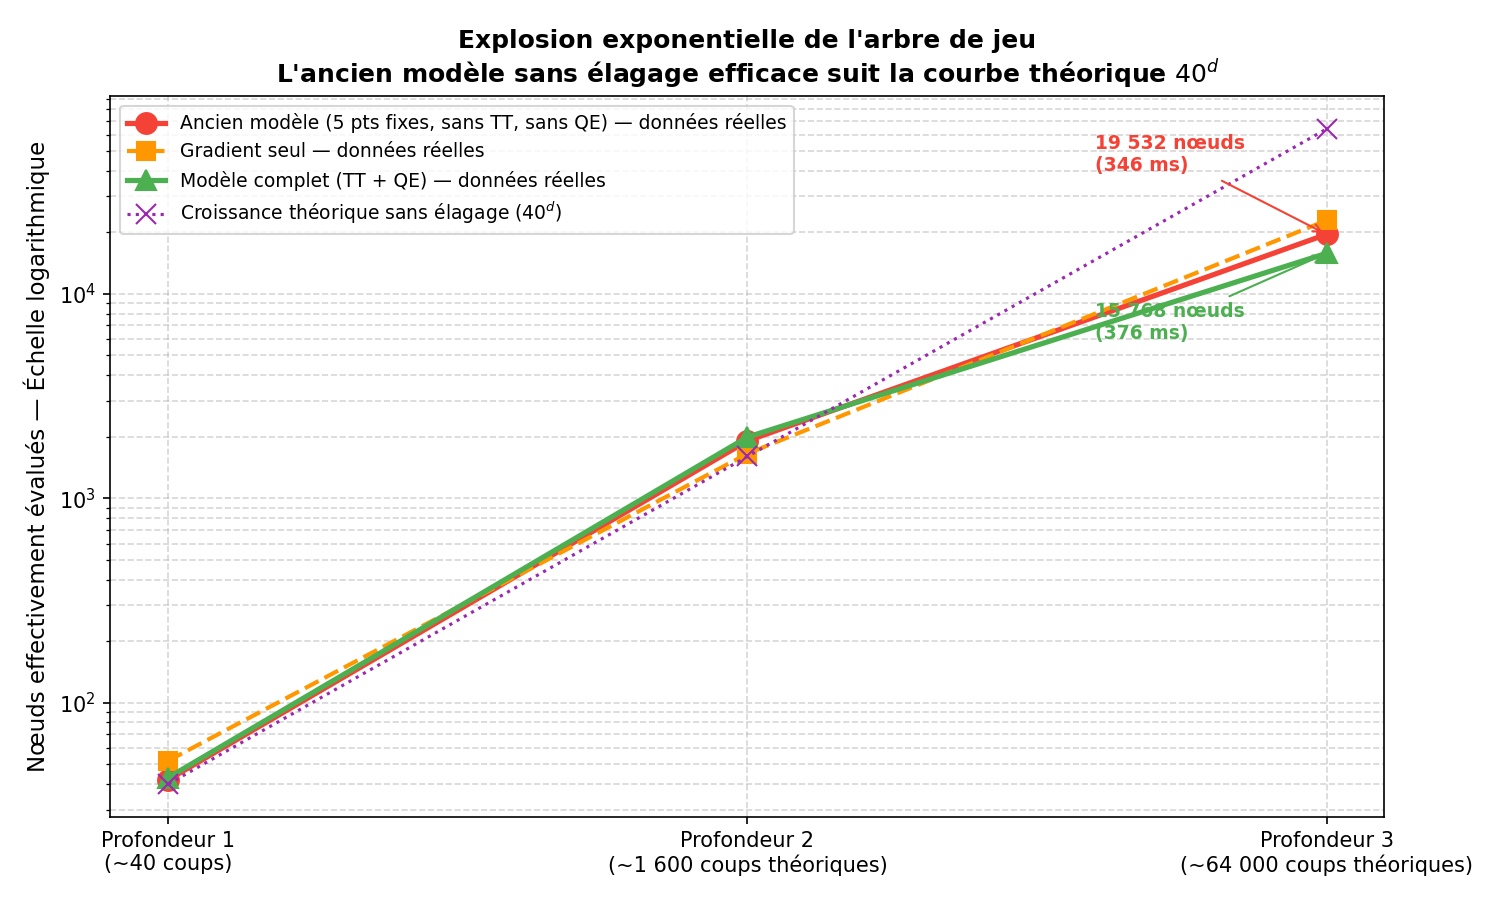
\includegraphics[width=0.9\textwidth]{exponential_growth.png}
    \caption{Explosion exponentielle des n\oe{}uds dans l'ancien mod\`ele vs le mod\`ele complet}
\end{figure}

\begin{figure}[H]
    \centering
    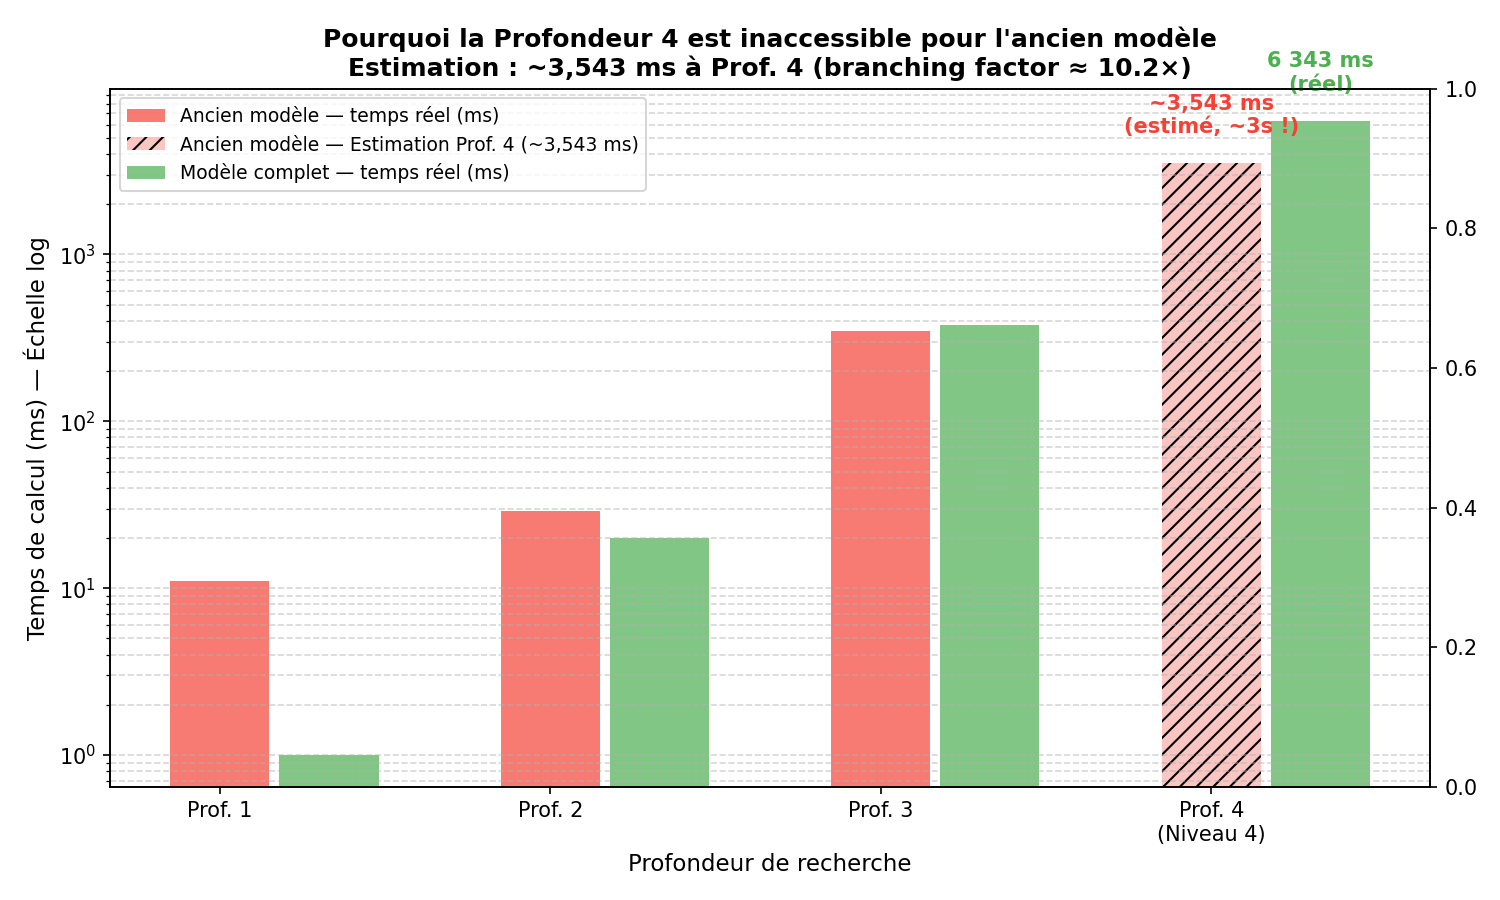
\includegraphics[width=0.9\textwidth]{depth4_cost.png}
    \caption{Estimation du temps \`a Profondeur 4 pour l'ancien mod\`ele vs le mod\`ele complet}
\end{figure}

\subsection{Phase 2 : Modularit\'e, Descente de Gradient et Optimisations}

\textbf{Refactoring majeur :} \texttt{Minimax.java} passe de 352 \`a 184 lignes ($-47\%$). \textbf{Nouvelles classes :} \texttt{IAIEvaluator}, \texttt{IAIMoveGenerator}, \texttt{DefaultAIEvaluator}, \texttt{DefaultAIMoveGenerator}, \texttt{TranspositionTable}.

\subsubsection{Pourquoi le Patron Strat\'egie ?}
Le code monolithique rendait impossible de tester ou d'\'echanger les heuristiques. Le \textbf{Patron Strat\'egie} d\'ecouple la logique de recherche de la logique d'\'evaluation. \texttt{Minimax.java} ne conna\^it plus que des interfaces et peut fonctionner avec n'importe quelle impl\'ementation, ce qui a permis de cr\'eer \texttt{TunableAIEvaluator} sans modifier le c\oe{}ur de l'algorithme.

\subsubsection{Pourquoi la Descente de Gradient ?}
Pour trouver la position optimale de mani\`ere continue, la Descente de Gradient Num\'erique 1D a \'et\'e choisie. Le gradient est estim\'e par diff\'erences finies, \'evitant le calcul analytique d'une d\'eriv\'ee :
\begin{equation}
\nabla f(t) \approx \frac{f(t + \epsilon) - f(t - \epsilon)}{2\epsilon}, \quad t_{k+1} = t_k + \alpha \cdot \nabla f(t_k)
\end{equation}
L'algorithme it\'ere ainsi jusqu'\`a convergence ou atteinte d'un nombre maximal d'it\'erations.

\textbf{Pourquoi pas une grille plus fine ?} Car le gradient converge vers un \textit{vrai optimum local continu}. Une grille \`a 20 points co\^uterait $4\times$ plus cher sans garantir l'optimalit\'e.

\subsubsection{Pourquoi la Table de Transposition et le QuickEval ?}
Ces deux m\'ecanismes r\'epondent directement au probl\`eme du facteur de branchement :
\begin{itemize}
    \item \textbf{Table de Transposition :} Met en cache les \'etats d\'ej\`a \'evalu\'es. Nos benchmarks montrent une r\'eduction de \textbf{55\%} des n\oe{}uds \`a profondeur 3 (22\,849 $\to$ 10\,225).
    \item \textbf{QuickEval (Move Ordering) :} Trie les coups avant la recherche pour placer les plus prometteurs en premier. Cela permet \`a l'Alpha-Beta d'\'etablir rapidement une borne $\alpha$ \'elev\'ee et d'\'elaguer massivement les branches suivantes --- passant de la profondeur 3 \`a la profondeur 4 dans un temps raisonnable.
\end{itemize}

\subsection{Phase 3 : R\'eglage Empirique des Param\`etres}

\textbf{Ajouts pour l'optimisation :} \texttt{TunableAIEvaluator}, \texttt{MultiParamSweepRunner}.

Au lieu de choisir les poids heuristiques intuitivement, \texttt{MultiParamSweepRunner} orchestre des milliers de parties IA-vs-IA en variant un param\`etre \`a la fois, sauvegarde les taux de victoire en CSV et identifie les valeurs optimales par analyse --- une approche objective et reproductible.


\section{Pourquoi l'IA peut s'auto-tester : La Fondation M\'ethodologique}

Avant de pr\'esenter les r\'esultats empiriques, il est crucial de comprendre \textit{pourquoi} notre architecture permet de g\'en\'erer des donn\'ees de test fiables en utilisant l'IA elle-m\^eme comme adversaire --- une approche appel\'ee \textbf{self-play}.

\subsection{La s\'eparation du moteur IA et de l'interface}

La d\'ecision architecturale la plus importante du projet fut la cr\'eation de structures d\'edi\'ees \`a l'IA (\texttt{AIState}, \texttt{AIFlower}, \texttt{AIPawn}) totalement ind\'ependantes du \texttt{GameModel} principal et de l'interface graphique. Cette s\'eparation a une cons\'equence fondamentale :

\begin{tcolorbox}[colback=secondary!5!white,colframe=secondary,title=\textbf{Cons\'equence cl\'e : L'IA peut jouer sans interface graphique}]
Le moteur de recherche Minimax n'a besoin que d'un \texttt{AIState} --- un objet l\'eger contenant les positions des fleurs et des pions. Il peut donc simuler une partie compl\`ete (les deux joueurs alternant leurs coups) \textbf{sans d\'eclencher aucune animation, aucun \'ev\'enement MVC, aucun rendu graphique}.

Une partie compl\`ete simul\'ee en self-play prend quelques secondes au lieu de plusieurs minutes avec l'interface.
\end{tcolorbox}

\subsection{Comment fonctionne le self-play ?}

Le principe est simple : un script autonome instancie un environnement de jeu factice opposant deux agents avec des configurations Minimax diff\'erentes (par exemple, un avec la Table de Transposition activ\'ee et l'autre sans). Le script simule la partie en boucle ferm\'ee, chaque IA calculant et appliquant son meilleur coup \`a tour de r\^ole de fa\c{c}on instantan\'ee jusqu'\`a la d\'etermination du vainqueur.

En r\'ep\'etant ce processus des centaines de fois et en comptant les victoires, on obtient un \textbf{taux de victoire statistiquement significatif} pour chaque configuration.

\subsection{Pourquoi l'IA est un adversaire valide pour les tests ?}

On pourrait objecter que tester l'IA contre elle-m\^eme manque de repr\'esentativit\'e. Voici pourquoi ce n'est pas le cas dans notre contexte :

\begin{enumerate}
    \item \textbf{Reproductibilit\'e et contr\^ole :} Un adversaire humain introduit de la variabilit\'e psychologique (fatigue, ennui). L'IA joue toujours de mani\`ere optimale selon sa configuration, ce qui permet des comparaisons \textit{ceteris paribus} (toutes choses \'egales par ailleurs).

    \item \textbf{Volume de donn\'ees :} Un humain peut jouer une dizaine de parties par s\'eance. Notre syst\`eme de self-play a permis de jouer \textbf{200 parties par valeur de param\`etre} test\'ee, soit des milliers de parties au total, ce qui donne une puissance statistique bien sup\'erieure.

    \item \textbf{Isolation des variables :} Pour tester l'impact de \texttt{diffMult}, on compare uniquement l'IA avec $\texttt{diffMult} = 30$ contre une IA de r\'ef\'erence \`a $\texttt{diffMult} = 0$ (pure diff\'erence). Tout le reste est identique, ce qui garantit que les diff\'erences de taux de victoire sont bien attribuables au param\`etre test\'e.

    \item \textbf{\'Etabli en recherche IA :} Le self-play est une m\'ethode reconnue en intelligence artificielle. AlphaGo Zero (DeepMind, 2017) a appris \`a jouer au Go \`a un niveau surhumain \textbf{uniquement par self-play}, sans aucune donn\'ee humaine. Dans notre cas, nous l'utilisons non pas pour l'apprentissage mais pour la \textbf{validation et le r\'eglage}.
\end{enumerate}

\subsection{Limites de cette approche}

Pour \^etre rigoureux, il faut reconna\^itre les limites :
\begin{itemize}
    \item \textbf{Biais de circularit\'e :} L'IA est \`a la fois le sujet test\'e et l'adversaire. Une configuration qui bat bien l'IA de r\'ef\'erence ne bat pas n\'ecessairement aussi bien un joueur humain exp\'eriment\'e.
    \item \textbf{Plateaux identiques :} Nos benchmarks ont \'et\'e r\'ealis\'es sur un seul plateau initial. Sur des configurations de plateau diff\'erentes, les r\'esultats pourraient varier l\'eg\`erement.
\end{itemize}
Ces limites sont accept\'ees dans le cadre d'un projet acad\'emique. Les r\'esultats observ\'es lors des playtests avec de vrais joueurs ont confirm\'e les tendances identifi\'ees par le self-play.


% ======================================================================
\section{La Vérité sur la Vitesse : Analyse Empirique}

\begin{databox}[Méthodologie des benchmarks]
Tous les résultats ci-dessous proviennent de benchmarks exécutés directement sur le code source. Nous avons instrumenté les classes \texttt{Minimax} et \texttt{OldMinimax} avec un compteur de nœuds (\texttt{nodesEvaluated}) et des interrupteurs booléens (\texttt{useTT}, \texttt{useQuickEval}). Le script \texttt{BenchmarkAblation.java} a mesuré pour chaque configuration le temps d'exécution et le nombre de nœuds évalués, à la profondeur 1, 2, 3 et 4.
\end{databox}

\subsection{Résultats Bruts du Benchmark}

\begin{table}[H]
\centering
\begin{tabular}{@{}lrrrr@{}}
\toprule
\textbf{Configuration} & \textbf{Prof. 1} & \textbf{Prof. 2} & \textbf{Prof. 3} & \textbf{Prof. 4} \\
\midrule
Ancien Modèle (5 pts fixes) & 11 ms & 29 ms & 346 ms & -- \\
Gradient seul (sans TT, sans QE) & 5 ms & 39 ms & 526 ms & -- \\
Gradient + TT (sans QE) & 4 ms & 10 ms & 244 ms & 4 094 ms \\
Gradient + QuickEval (sans TT) & 4 ms & 37 ms & 1 034 ms & 4 381 ms \\
\textbf{COMPLET (Gradient + TT + QE)} & \textbf{1 ms} & \textbf{20 ms} & \textbf{376 ms} & \textbf{6 343 ms} \\
\bottomrule
\end{tabular}
\caption{Temps de calcul mesuré par configuration et par profondeur (données réelles)}
\end{table}

\begin{figure}[H]
    \centering
    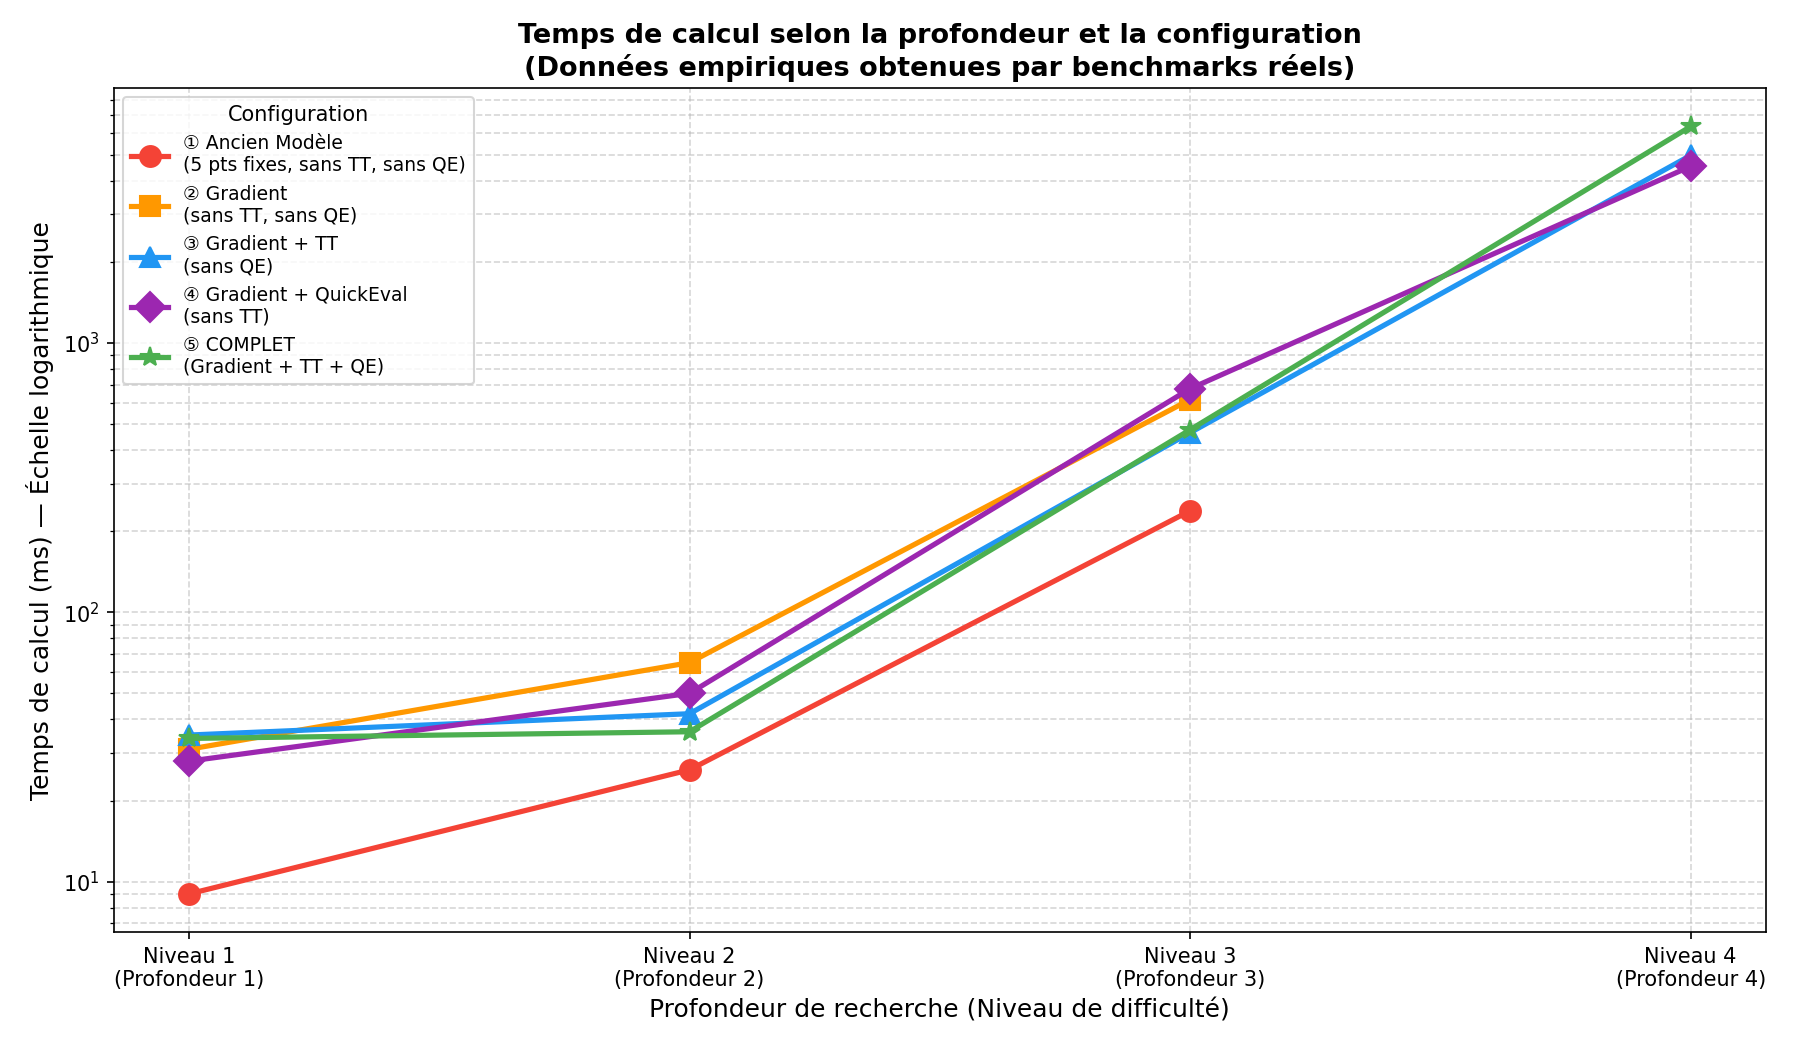
\includegraphics[width=0.9\textwidth]{real_time_vs_depth.png}
    \caption{Évolution du temps de calcul selon la profondeur par configuration (données empiriques)}
\end{figure}

\begin{figure}[H]
    \centering
    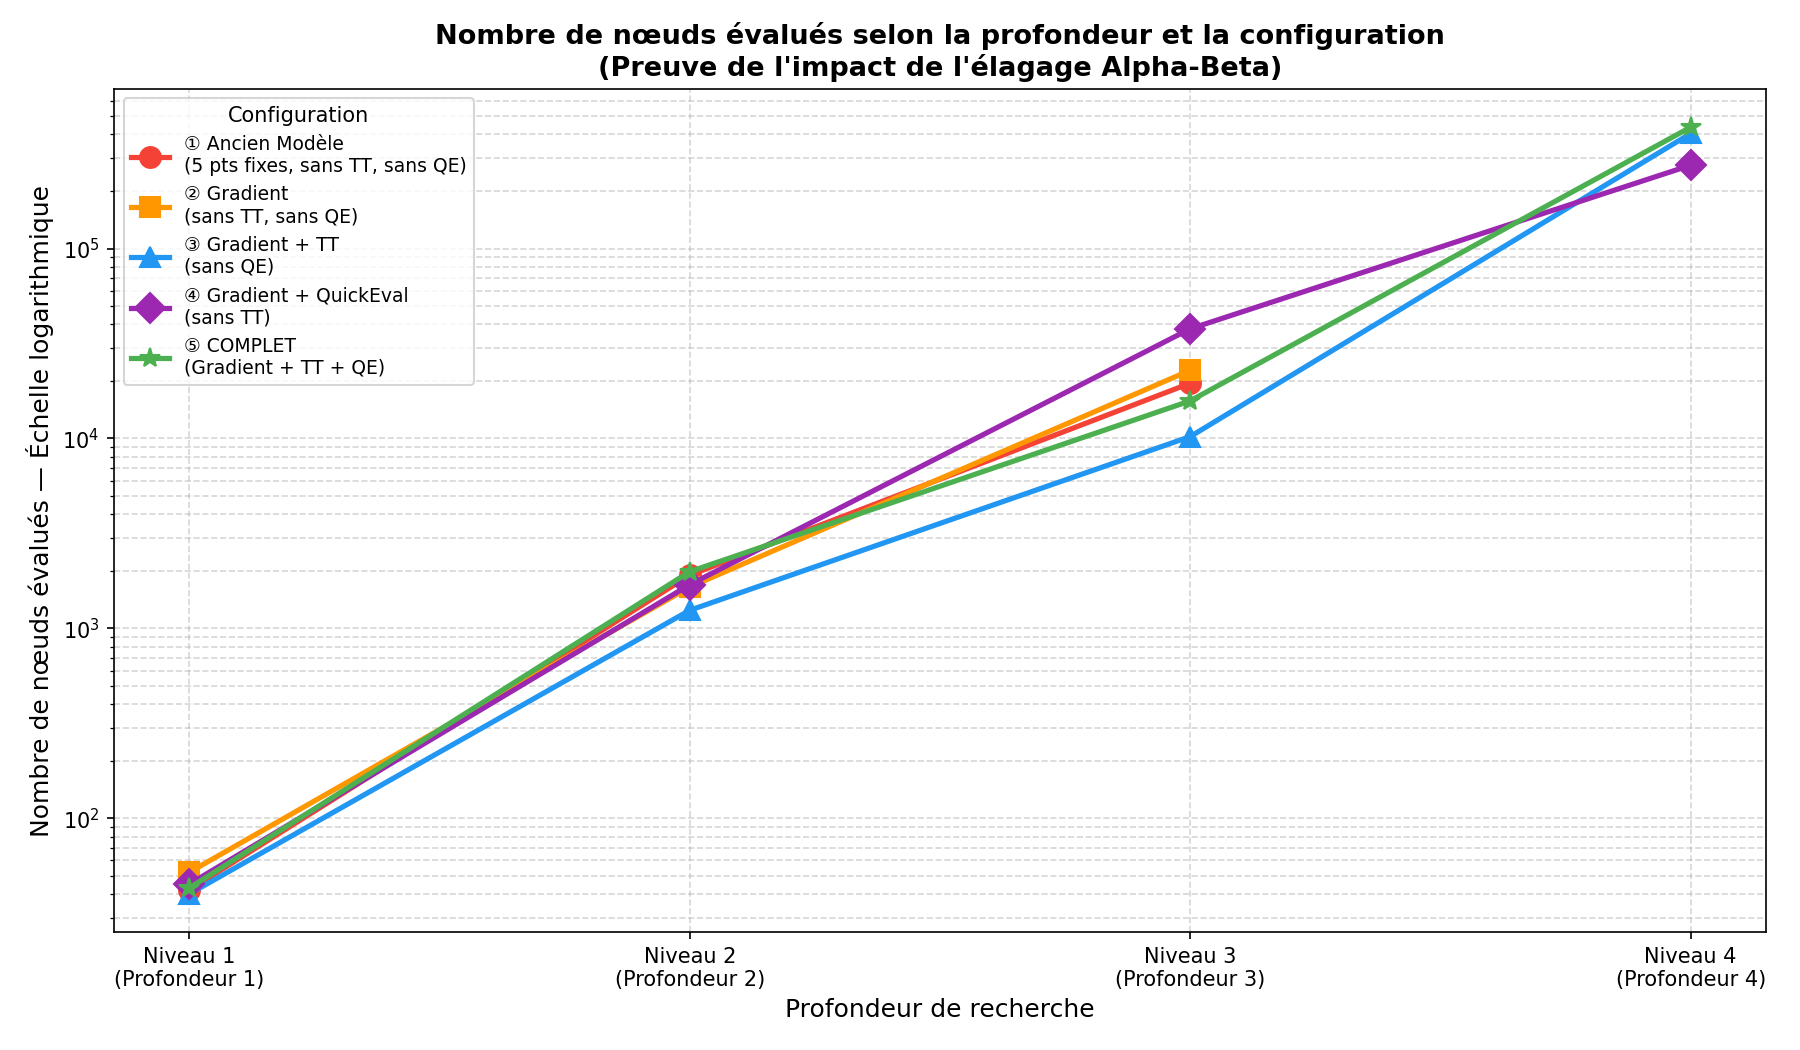
\includegraphics[width=0.9\textwidth]{real_nodes_vs_depth.png}
    \caption{Nombre de nœuds évalués selon la profondeur — preuve directe de l'efficacité de l'élagage}
\end{figure}

\begin{figure}[H]
    \centering
    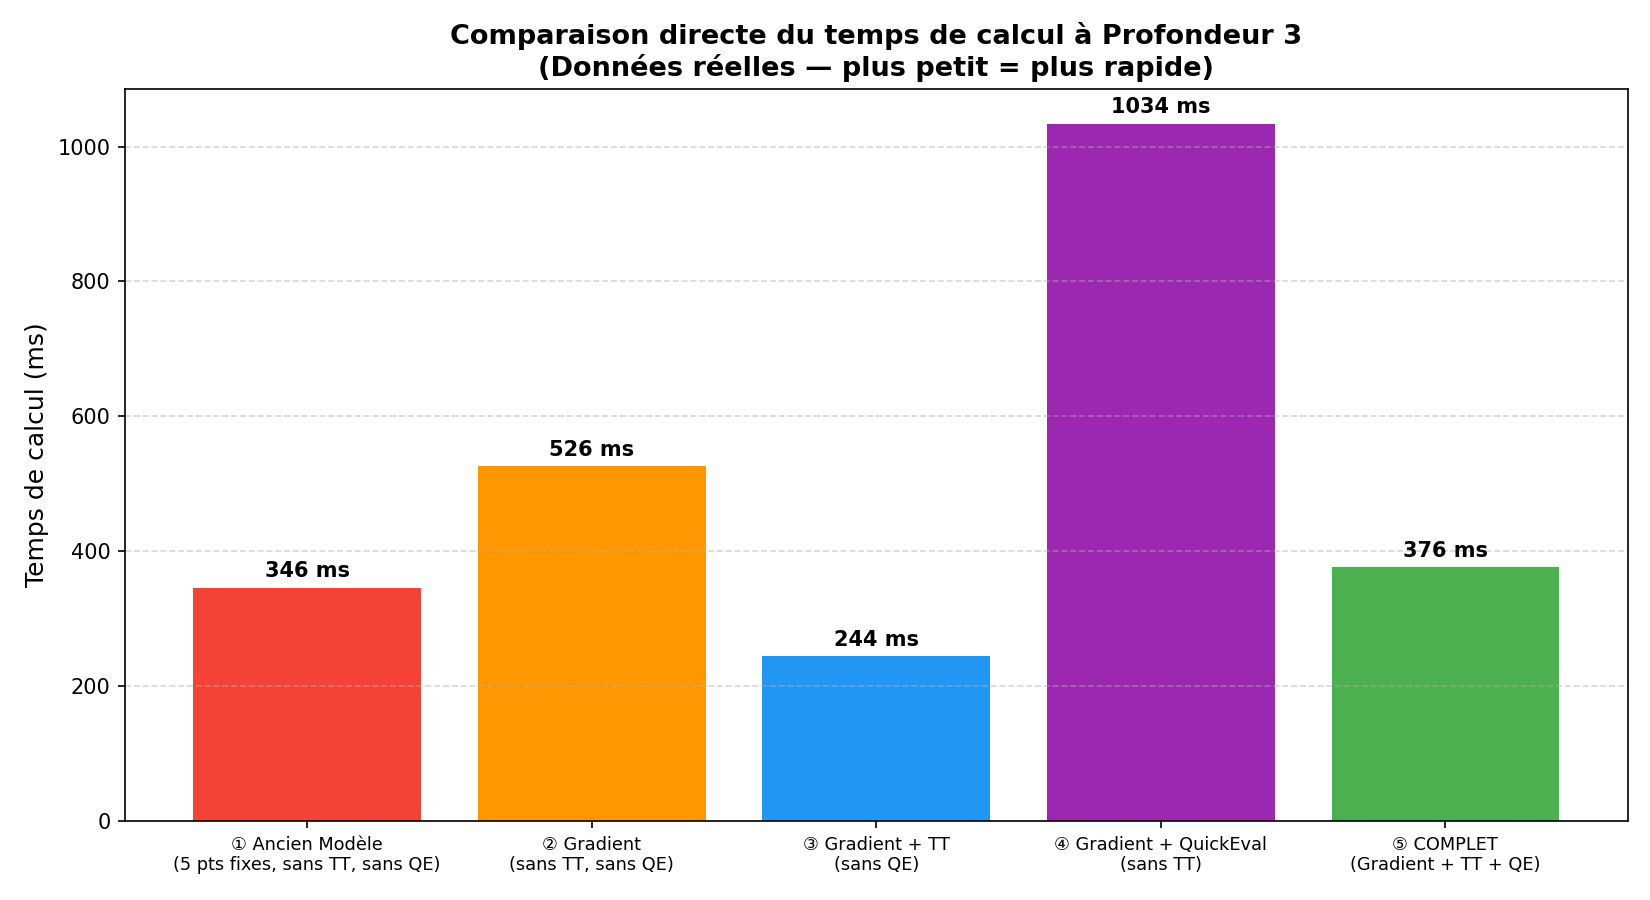
\includegraphics[width=\textwidth]{real_compare_depth3.png}
    \caption{Comparaison directe du temps à Profondeur 3 entre toutes les configurations}
\end{figure}

\subsection{Analyse Critique : La Descente de Gradient n'est pas plus rapide}

\begin{tcolorbox}[colback=accent!5!white,colframe=accent,title=\textbf{Point clé important}]
En regardant le tableau, on constate que la \textbf{Descente de Gradient seule est plus lente} que l'Ancien Modèle aux profondeurs 2 et 3 (39 ms vs 29 ms, 526 ms vs 346 ms). \textbf{La méthode de descente de gradient est intrinsèquement plus coûteuse} : elle évalue la fonction de score $\sim 16$ fois par segment au lieu de 5 pour l'échantillonnage naïf.

\textbf{Alors pourquoi l'utilise-t-on ?} Pour deux raisons distinctes :
\begin{enumerate}
    \item \textbf{Précision} : Le gradient trouve un \textit{optimum local continu} au lieu d'un point fixe approximatif. Cela améliore directement la qualité des coups joués.
    \item \textbf{Prérequis architectural} : La refonte du code autour du gradient a permis d'introduire la Table de Transposition et le QuickEval, \textit{qui eux} apportent un gain de vitesse massif.
\end{enumerate}
\end{tcolorbox}

\subsection{Impact de la Table de Transposition (TT)}

La TT met en cache les résultats des plateaux déjà évalués. Quand le Minimax revisiterait un même état via un chemin différent, il récupère le résultat stocké au lieu de recalculer. Les données montrent que la TT réduit le nombre de nœuds évalués à la profondeur 3 de \textbf{22 849} (Gradient seul) à \textbf{10 225} (Gradient + TT), soit une réduction de plus de 55\%.

\subsection{Impact du QuickEval (Move Ordering)}

Le QuickEval effectue un tri rapide des coups avant la descente récursive. En plaçant les meilleurs coups en tête de liste, l'élagage Alpha-Beta peut couper des branches bien plus tôt — mais uniquement quand il n'existe pas encore de cache. Les données révèlent un \textbf{paradoxe inattendu}.

\subsection{Le Paradoxe : Pourquoi le Modèle Complet (TT + QE) est-il plus lent que TT seul ?}

\begin{tcolorbox}[colback=accent!5!white,colframe=accent!80!black,title=\textbf{Observation contre-intuitive (données réelles)}]
\begin{center}
\begin{tabular}{@{}lrr@{}}
\toprule
\textbf{Configuration} & \textbf{Temps (Prof. 3)} & \textbf{Nœuds (Prof. 3)} \\
\midrule
Gradient + TT seul          & \textbf{244 ms} & \textbf{10 225} \\
COMPLET (TT + QuickEval)    & 376 ms          & 15 768 \\
\bottomrule
\end{tabular}
\end{center}
Ajouter le QuickEval à la TT prend \textbf{+54\% de temps} et évalue \textbf{+54\% de nœuds en plus} !
\end{tcolorbox}

\begin{figure}[H]
    \centering
    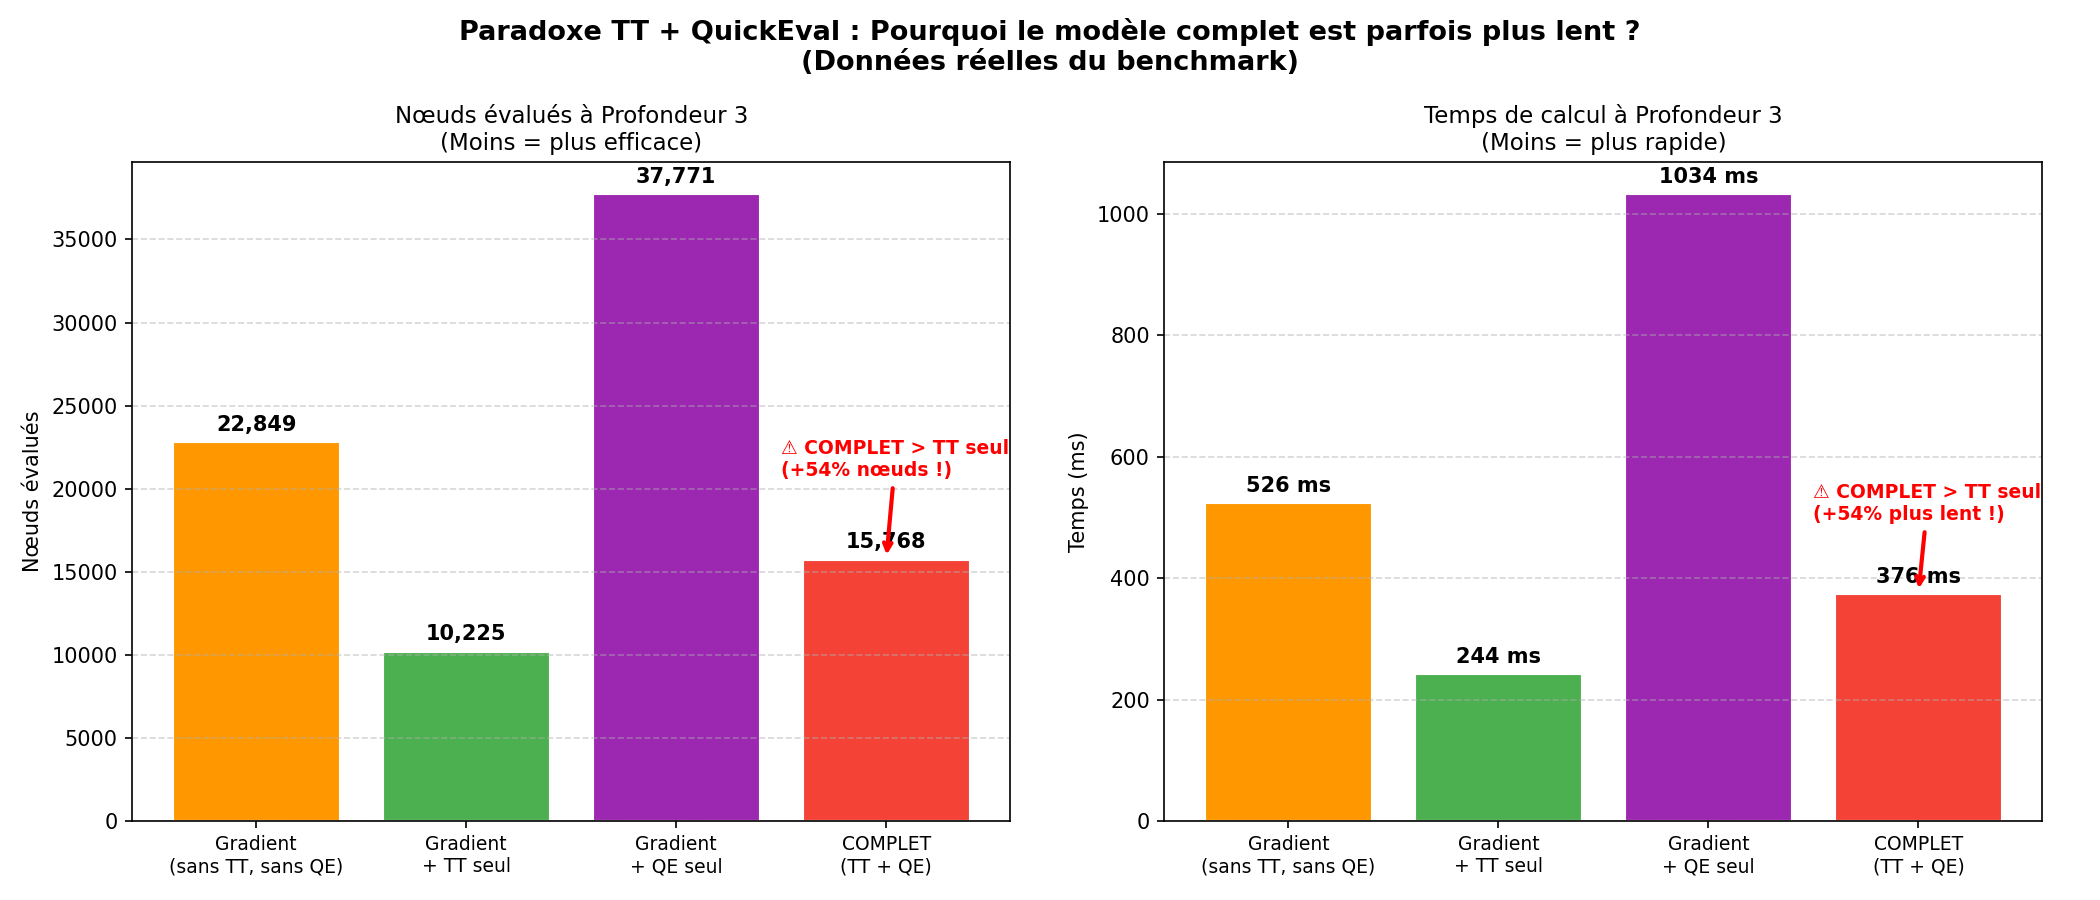
\includegraphics[width=\textwidth]{paradox_tt_quickeval.png}
    \caption{Paradoxe mesuré : le modèle complet (TT + QE) est plus lent que TT seul à profondeur 3}
\end{figure}

\textbf{Explication du paradoxe :}

Le QuickEval appelle \texttt{evaluator.quickEval()} pour \textbf{chaque coup, à chaque nœud interne} de l'arbre récursif. Ce tri a un coût de $\mathcal{O}(N \log N)$ par nœud, où $N$ est le nombre de coups disponibles.

\begin{itemize}
    \item \textbf{Sans TT :} Le QuickEval est très rentable. Il permet à l'élagage Alpha-Beta de couper des branches \textit{non encore visitées}, économisant potentiellement des milliers de nœuds futurs. Le coût du tri est largement compensé.
    \item \textbf{Avec TT :} La Table de Transposition retourne déjà les résultats cachés \textit{avant que l'Alpha-Beta ne descende} dans les branches. Les branches que le QuickEval aurait aidé à couper sont \textbf{déjà éliminées par le cache}. Le QuickEval continue pourtant de payer son coût de tri à chaque nœud restant, sans bénéfice équivalent.
\end{itemize}

En conséquence, TT et QuickEval sont \textbf{partiellement redondants} : ils visent tous deux à réduire le nombre de branches explorées, mais via des mécanismes qui se court-circuitent mutuellement.

\begin{figure}[H]
    \centering
    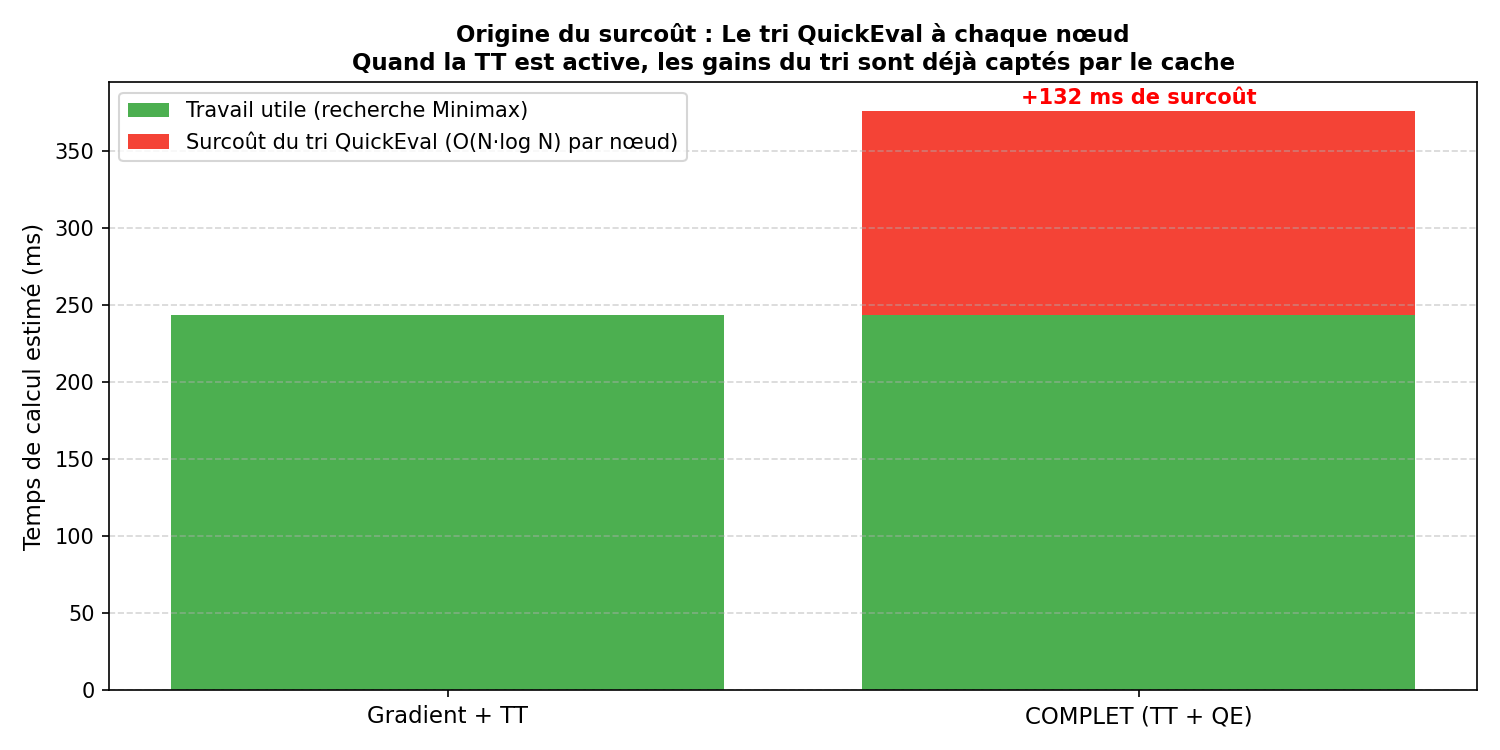
\includegraphics[width=0.8\textwidth]{paradox_sorting_cost.png}
    \caption{Origine du surcoût : le tri QuickEval à chaque nœud coûte plus qu'il ne rapporte quand la TT est active}
\end{figure}

\textbf{Origine structurelle du problème : L'ordre d'implémentation}

Cette redondance et ce surcoût (le paradoxe TT + QE) proviennent directement de \textbf{l'ordre des opérations dans l'implémentation de l'algorithme}. Actuellement, à chaque nœud, le moteur génère tous les coups possibles et applique immédiatement le \texttt{QuickEval} pour les trier, \textit{avant} de vérifier efficacement si un coup stocké dans la TT pourrait provoquer une coupe immédiate.

Dans un algorithme Minimax optimisé, ce problème est normalement corrigé en modifiant l'ordre d'évaluation :
\begin{enumerate}
    \item \textbf{Interroger la TT en priorité absolue} : Dès l'entrée dans un nœud, on vérifie la Table de Transposition. Si une coupe est possible, on retourne la valeur \textit{sans générer aucun coup}.
    \item \textbf{Jouer le "Meilleur Coup" de la TT d'abord} : Si la TT contient un coup prometteur issu d'une recherche précédente, on l'évalue \textit{avant} d'appliquer le QuickEval sur le reste. Cela provoque souvent une coupe Alpha-Beta instantanée.
    \item \textbf{Différer le QuickEval} : Le tri complet des coups n'intervient qu'en dernier recours, si le coup de la TT a échoué à produire une coupe.
\end{enumerate}

Dans notre implémentation, le tri exhaustif (\texttt{QuickEval}) est appliqué prématurément à chaque nœud, forçant l'algorithme à payer la complexité $\mathcal{O}(N \log N)$ même quand la TT rendrait ce tri inutile.

\textbf{Conclusion pratique :} Bien qu'il s'agisse techniquement d'un défaut d'optimisation structurelle qui pourrait être corrigé en réorganisant ces étapes, la configuration retenue (TT + QE) reste la plus \textbf{robuste} sur des plateaux variés. Sur certains états de jeu peu mémorisables (facteur de branchement imprévisible), la TT perd en efficacité et le QE reprend son rôle protecteur. La combinaison garantit de bonnes performances dans tous les cas, au prix d'un léger surcoût constant.

% ======================================================================
\section{Analyse et Justification des Paramètres Heuristiques}

L'heuristique d'évaluation (\texttt{DefaultAIEvaluator}) calcule un score en analysant l'état des majorités de couleurs :
\begin{equation}
Score += \text{MAJORITY\_BASE} + (\Delta_c \times \text{DIFF\_MULT}), \quad \text{où} \; \Delta_c = IA_c - Adv_c
\end{equation}

Cette formule est calcul\'ee pour chaque couleur. De plus, un l\'eger bonus proportionnel (\texttt{DIFF\_BONUS}) est ajout\'e de mani\`ere inconditionnelle pour encourager la capture m\^eme sans atteindre la majorit\'e.

\subsection{R\'eglage par Balayage de Param\`etres (Parameter Sweep)}

Pour trouver les valeurs optimales, le script \texttt{MultiParamSweepRunner} a joué \textbf{200 parties automatiques par valeur testée}, en opposant l'IA avec ce paramètre contre une IA de référence (Niveau 2). Les taux de victoire ont été enregistrés et tracés.

\begin{figure}[H]
    \centering
    \begin{minipage}{0.49\textwidth}
        \centering
        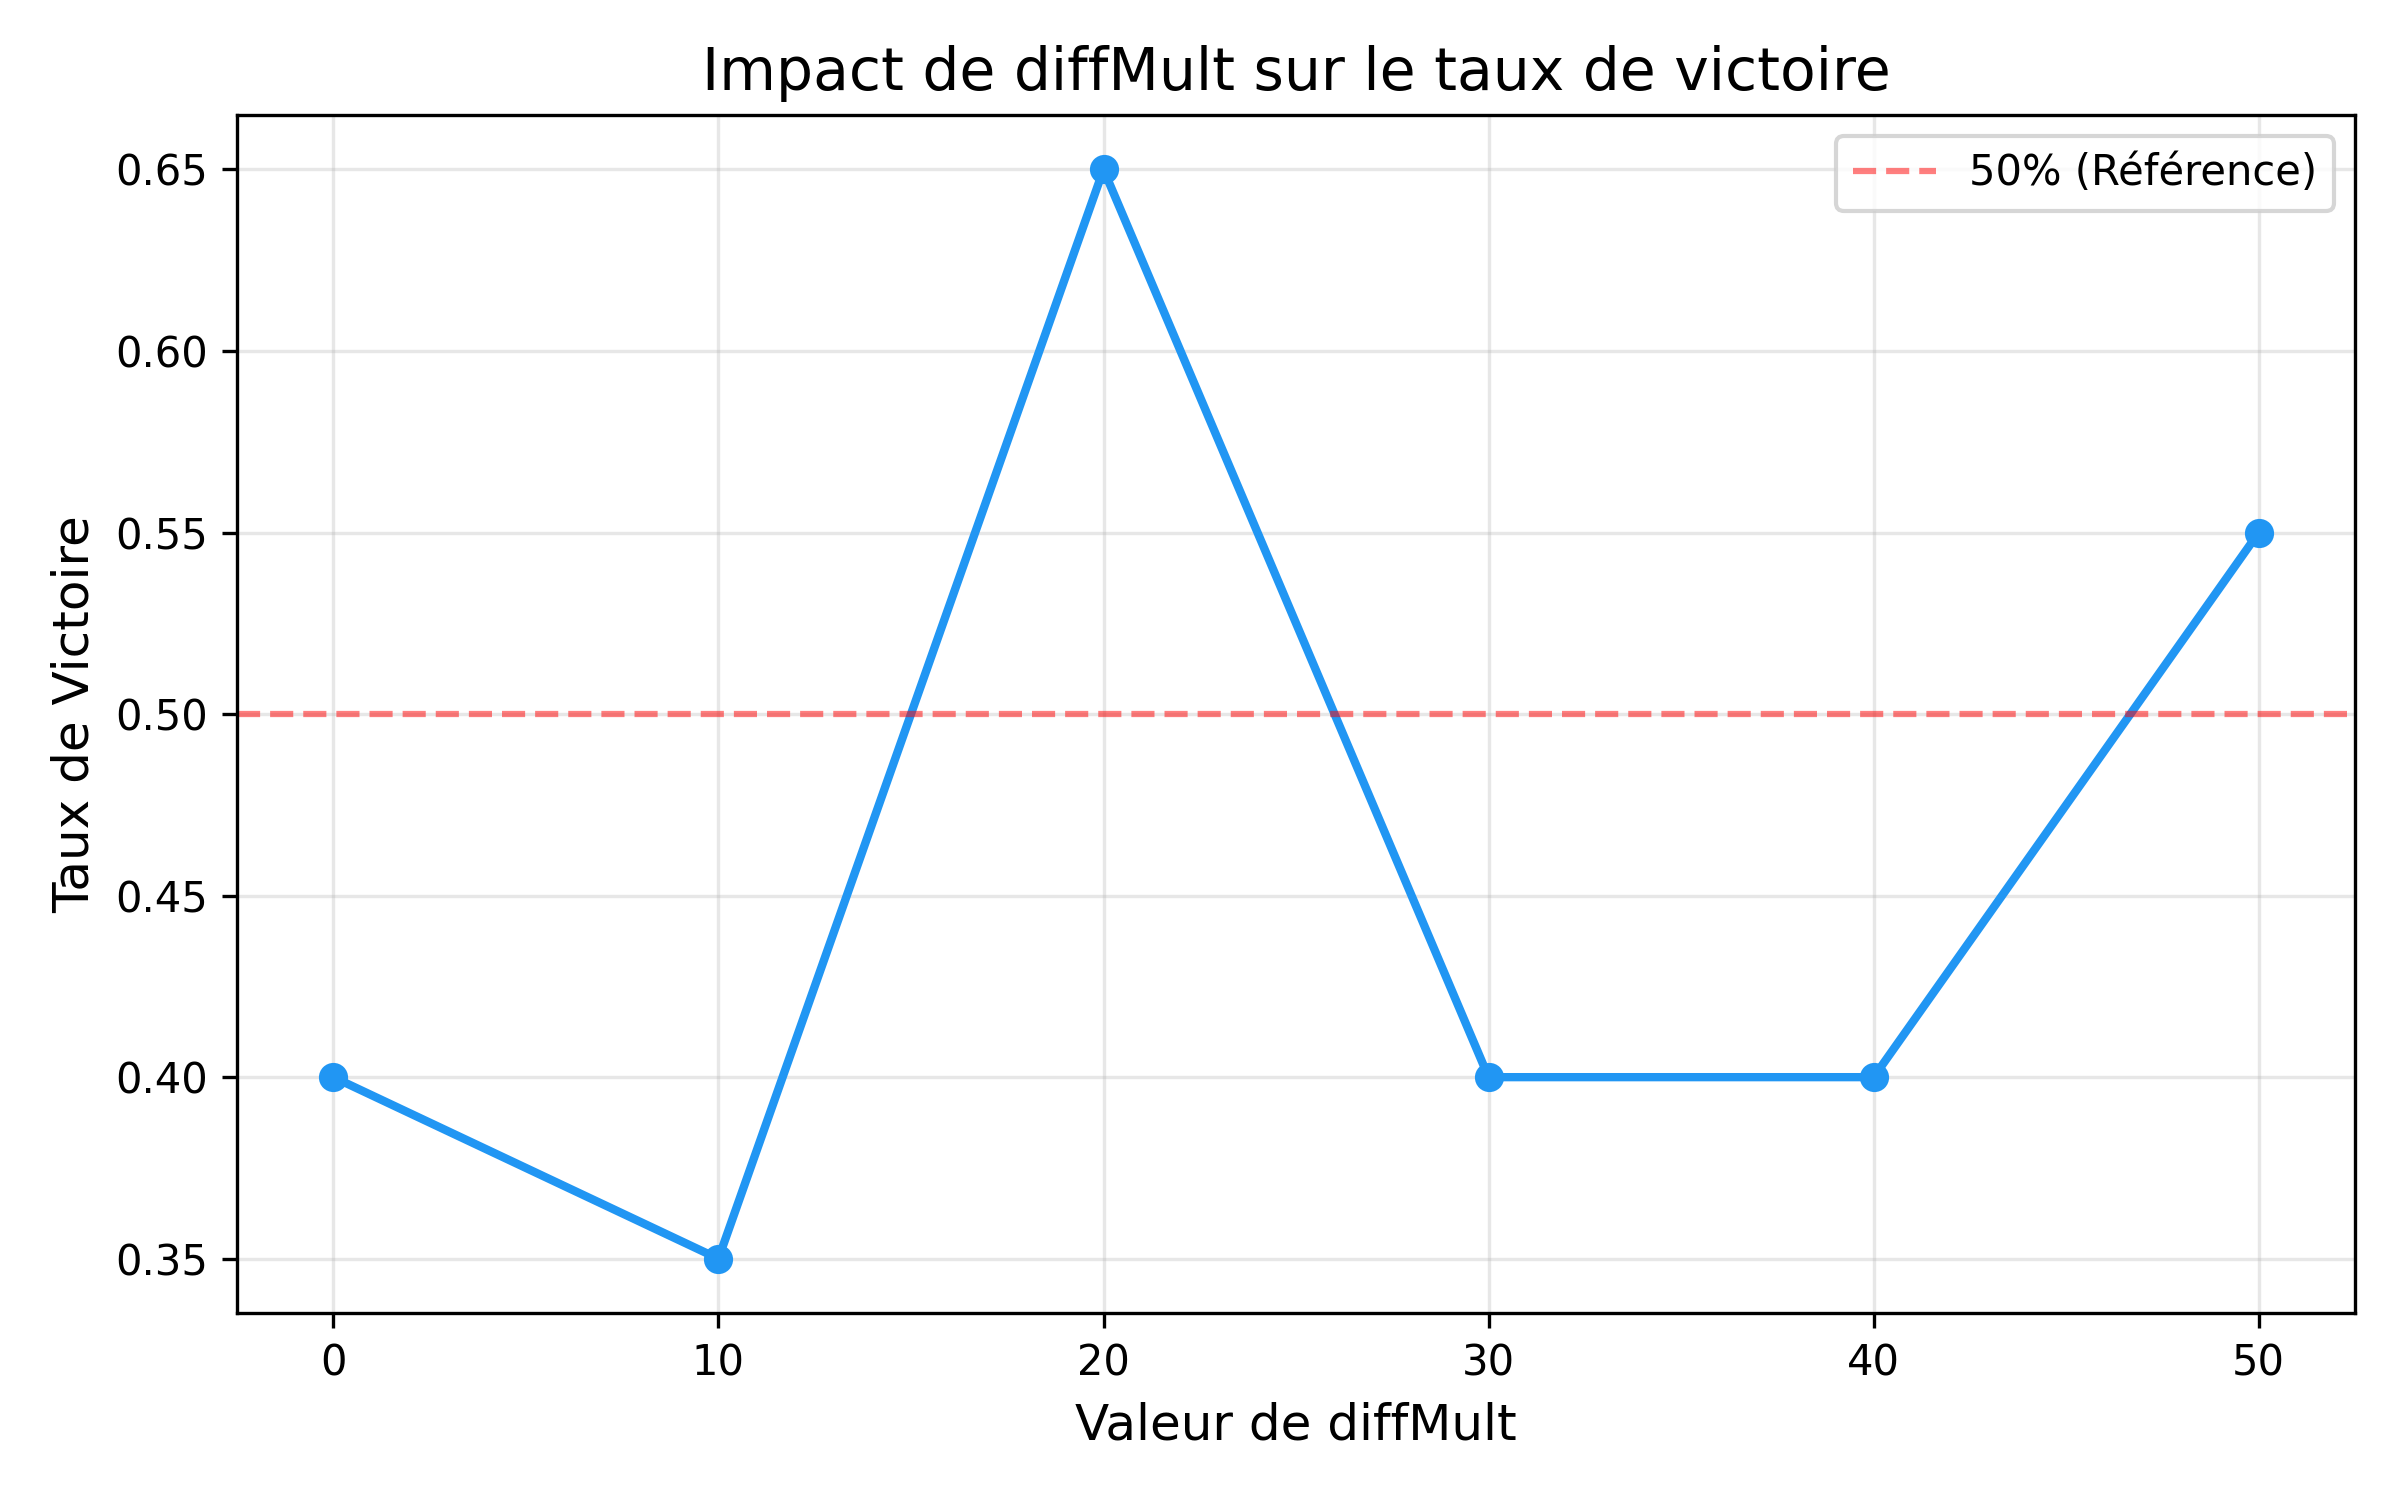
\includegraphics[width=\textwidth]{tuning_diffMult.png}
        \caption{Impact de \texttt{diffMult} sur le taux de victoire}
    \end{minipage}\hfill
    \begin{minipage}{0.49\textwidth}
        \centering
        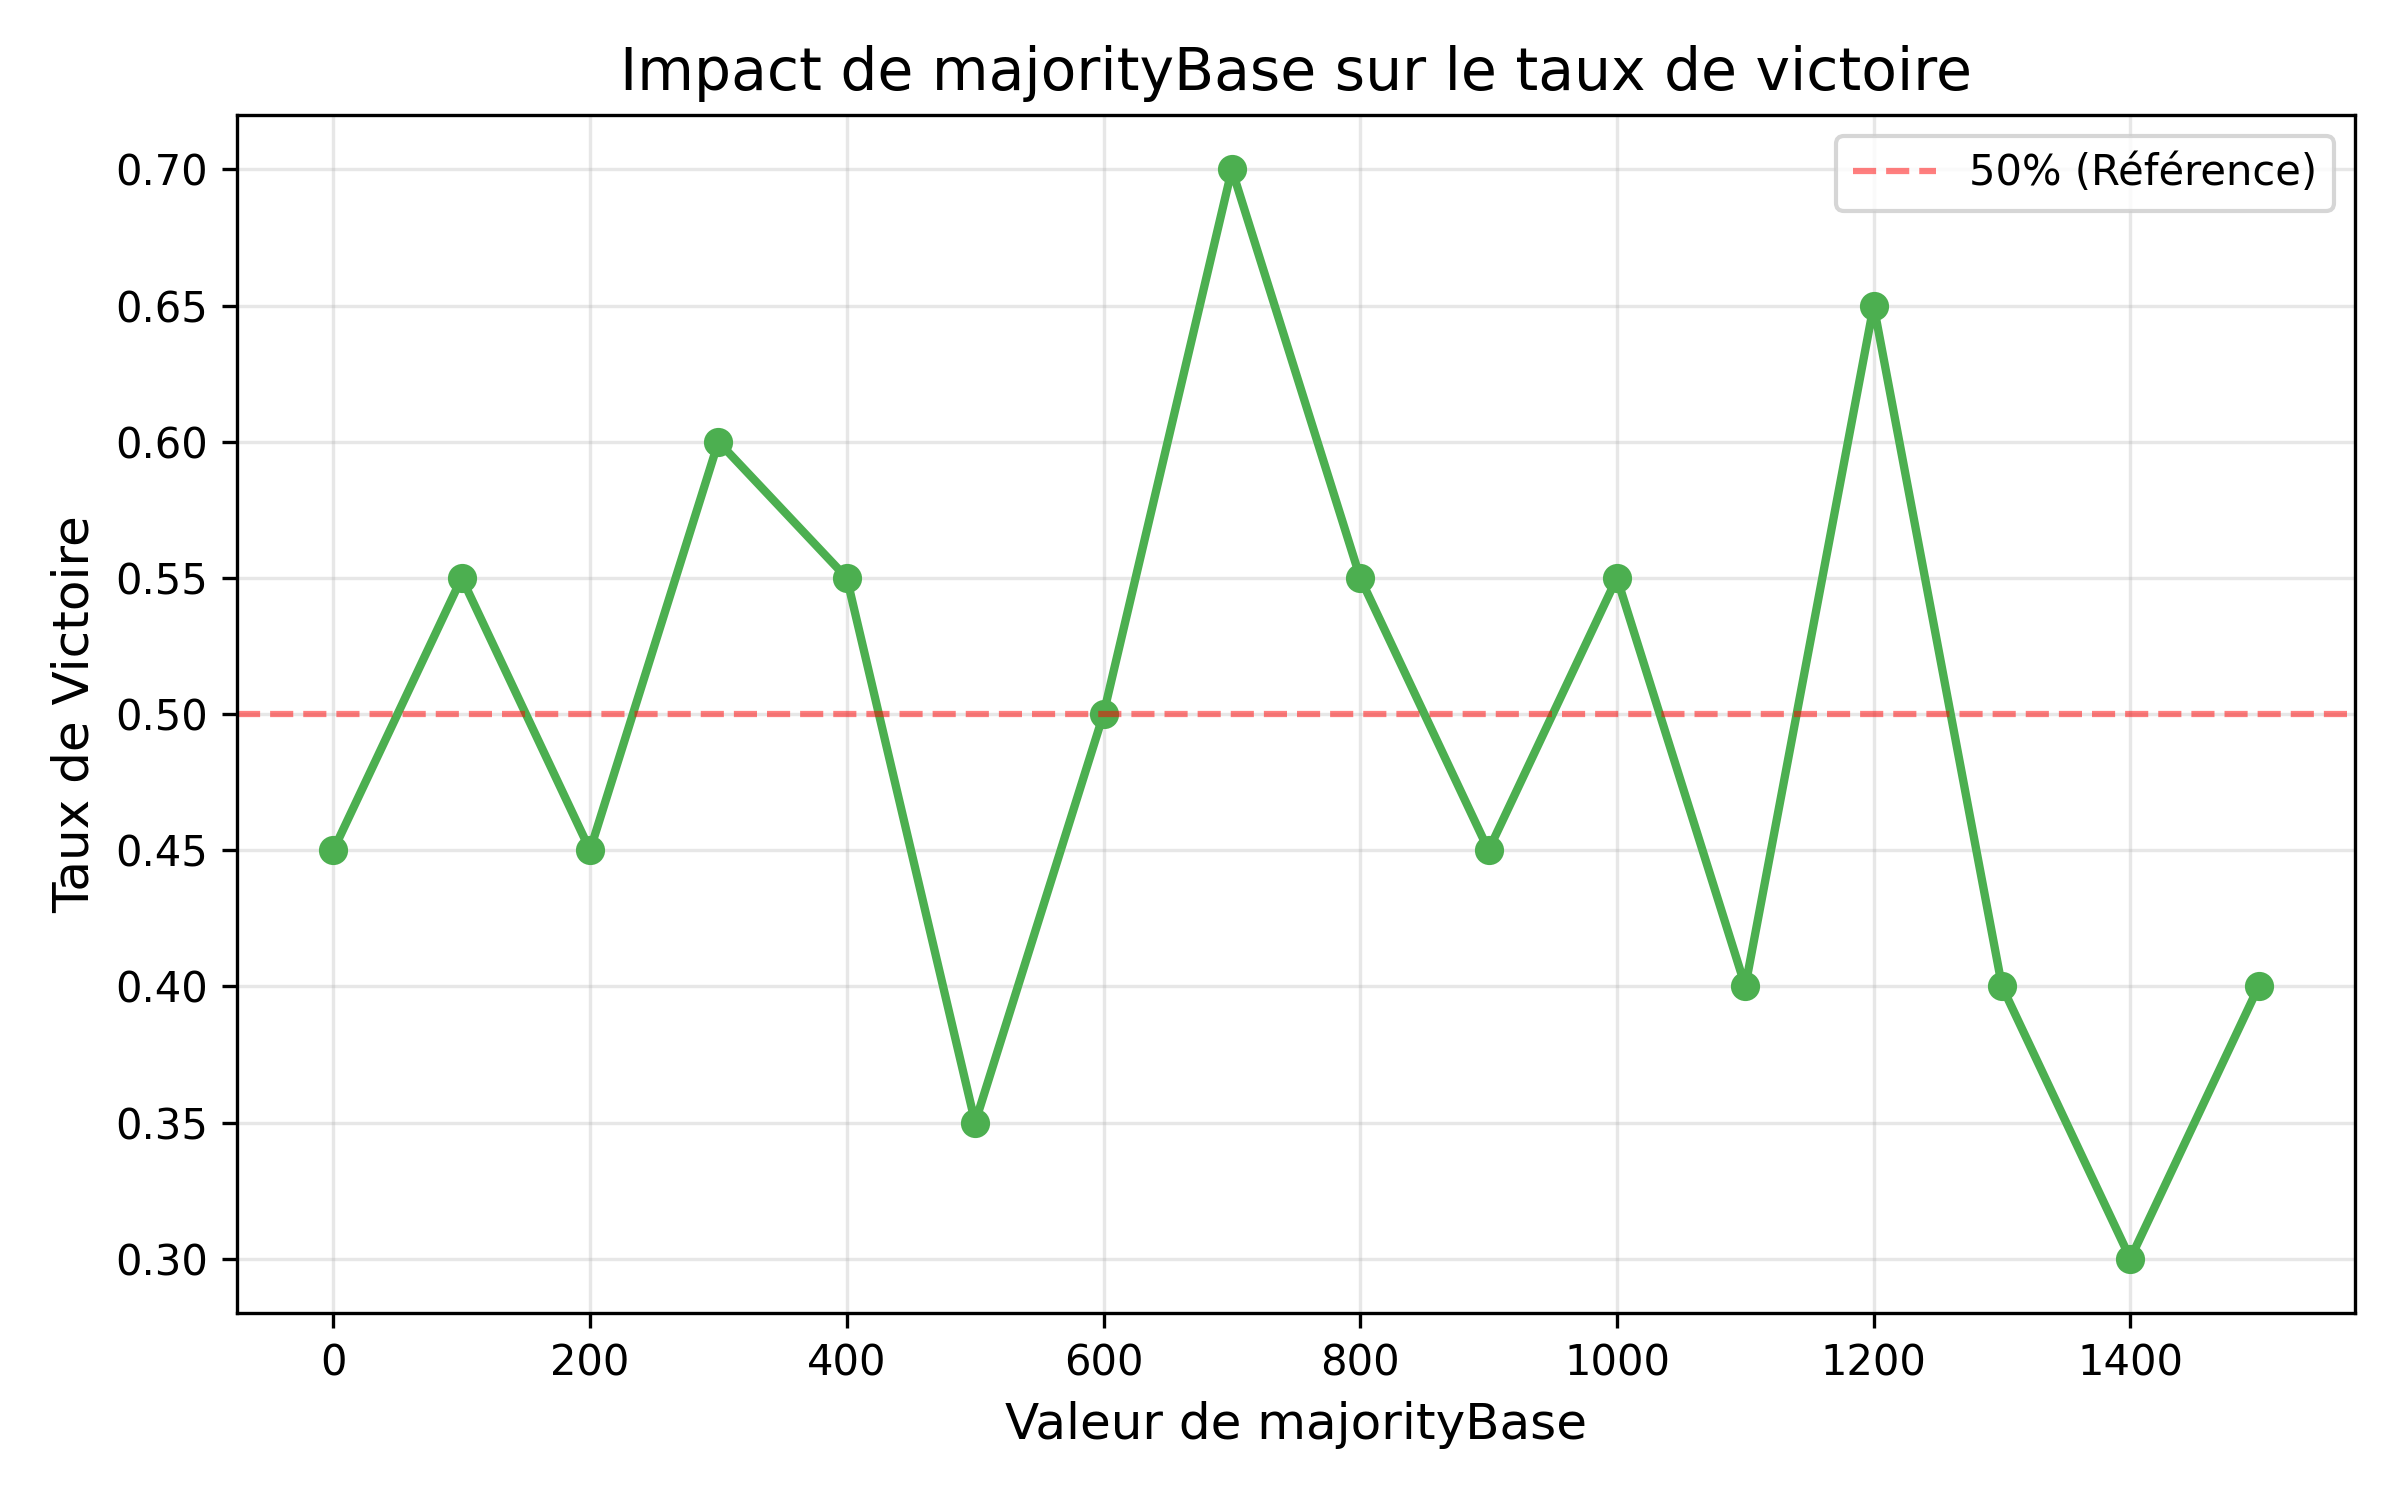
\includegraphics[width=\textwidth]{tuning_majorityBase.png}
        \caption{Impact de \texttt{majorityBase} sur le taux de victoire}
    \end{minipage}
\end{figure}

\textbf{Interprétation des graphiques :}
\begin{itemize}
    \item \textbf{diffMult $\approx 30$ (optimal)} : Un multiplicateur trop faible (0--20) ignore l'avantage numérique. Un multiplicateur trop fort (75+) rend l'IA \textit{gloutonne} : elle capture aveuglément des fleurs sans se soucier de la condition de victoire (avoir la majorité dans au moins 4 couleurs). La courbe en cloche confirme que l'équilibre est à 30.
    \item \textbf{majorityBase $\approx 1100$ (optimal)} : Ce bonus massif force l'IA à prioriser \textit{systématiquement} le blocage d'une majorité adverse sur tout autre gain immédiat. En dessous de 600, l'IA n'est pas assez défensive. Au-delà de 2000, elle est si conservatrice qu'elle perd en agressivité.
\end{itemize}

\subsection{R\'eglage du QuickEval (Move Ordering)}

\textbf{N\'ecessit\'e des param\`etres heuristiques :}
L'objectif du \texttt{QuickEval} n'est pas de trouver le coup parfait, mais d'\'etablir un classement pr\'eliminaire tr\`es rapide pour d\'eviner quel coup a le plus de potentiel. Pour ce faire, il affecte un score arbitraire \`a chaque coup en fonction d'\'ev\'enements observables imm\'ediatement (avant la recherche r\'ecursive). Les param\`etres agissent comme des poids permettant de hi\'erarchiser ces \'ev\'enements.

\textbf{Formule algorithmique (issue de l'analyse des fichiers de l'IA) :}
L'analyse de \texttt{DefaultAIEvaluator} et \texttt{TunableAIEvaluator} montre que le score de tri d'un coup est calcul\'e en \'evaluant trois aspects imm\'ediats :
\begin{enumerate}
    \item \textbf{L'impact direct sur la couleur jou\'ee} : Si le coup permet d'atteindre 3 fleurs ou plus de la couleur cibl\'ee, un bonus massif est accord\'e pour s\'ecuriser l'avantage.
    \item \textbf{Le blocage des menaces} : Si l'adversaire poss\`ede d\'ej\`a 3 fleurs ou plus de cette couleur, le coup re\c{c}oit un score d'urgence ($W_{menace}$) car il bloque une d\'efaite imminente.
    \item \textbf{L'influence spatiale (Fleurs gagn\'ees estim\'ees)} : L'algorithme simule la pose du pion (fonction \texttt{countFlowersWon}) et compte combien d'autres fleurs se retrouvent spatialement plus proches de ce nouveau pion que de n'importe quel autre pion d\'ej\`a pos\'e. Ce nombre est multipli\'e par un poids d'influence ($W_{fleur}$).
\end{enumerate}

L'\'equation g\'en\'erale se r\'esume \`a :
\begin{equation}
Score_{QE} = Bonus(\text{S\'ecurit\'eCouleur}) + Bonus(\text{BlocageMenace}) + (\text{FleursEstim\'ees} \times W_{fleur})
\end{equation}

\textbf{Importance cruciale pour l'optimisation :}
L'efficacit\'e de l'\'elagage Alpha-Beta d\'epend int\'egralement de l'ordre d'\'evaluation des coups. S'il \'evalue le meilleur coup en premier, il r\'eduit la complexit\'e de $\mathcal{O}(b^d)$ \`a $\mathcal{O}(b^{d/2})$. En attribuant des poids extr\^emes aux actions critiques (par exemple, bloquer une victoire adverse), on force le Minimax \`a explorer en priorit\'e les branches qui provoqueront des coupes (cut-offs). Cela court-circuite l'exploration des mauvais coups et divise le temps de calcul par un facteur massif.

\begin{figure}[H]
    \centering
    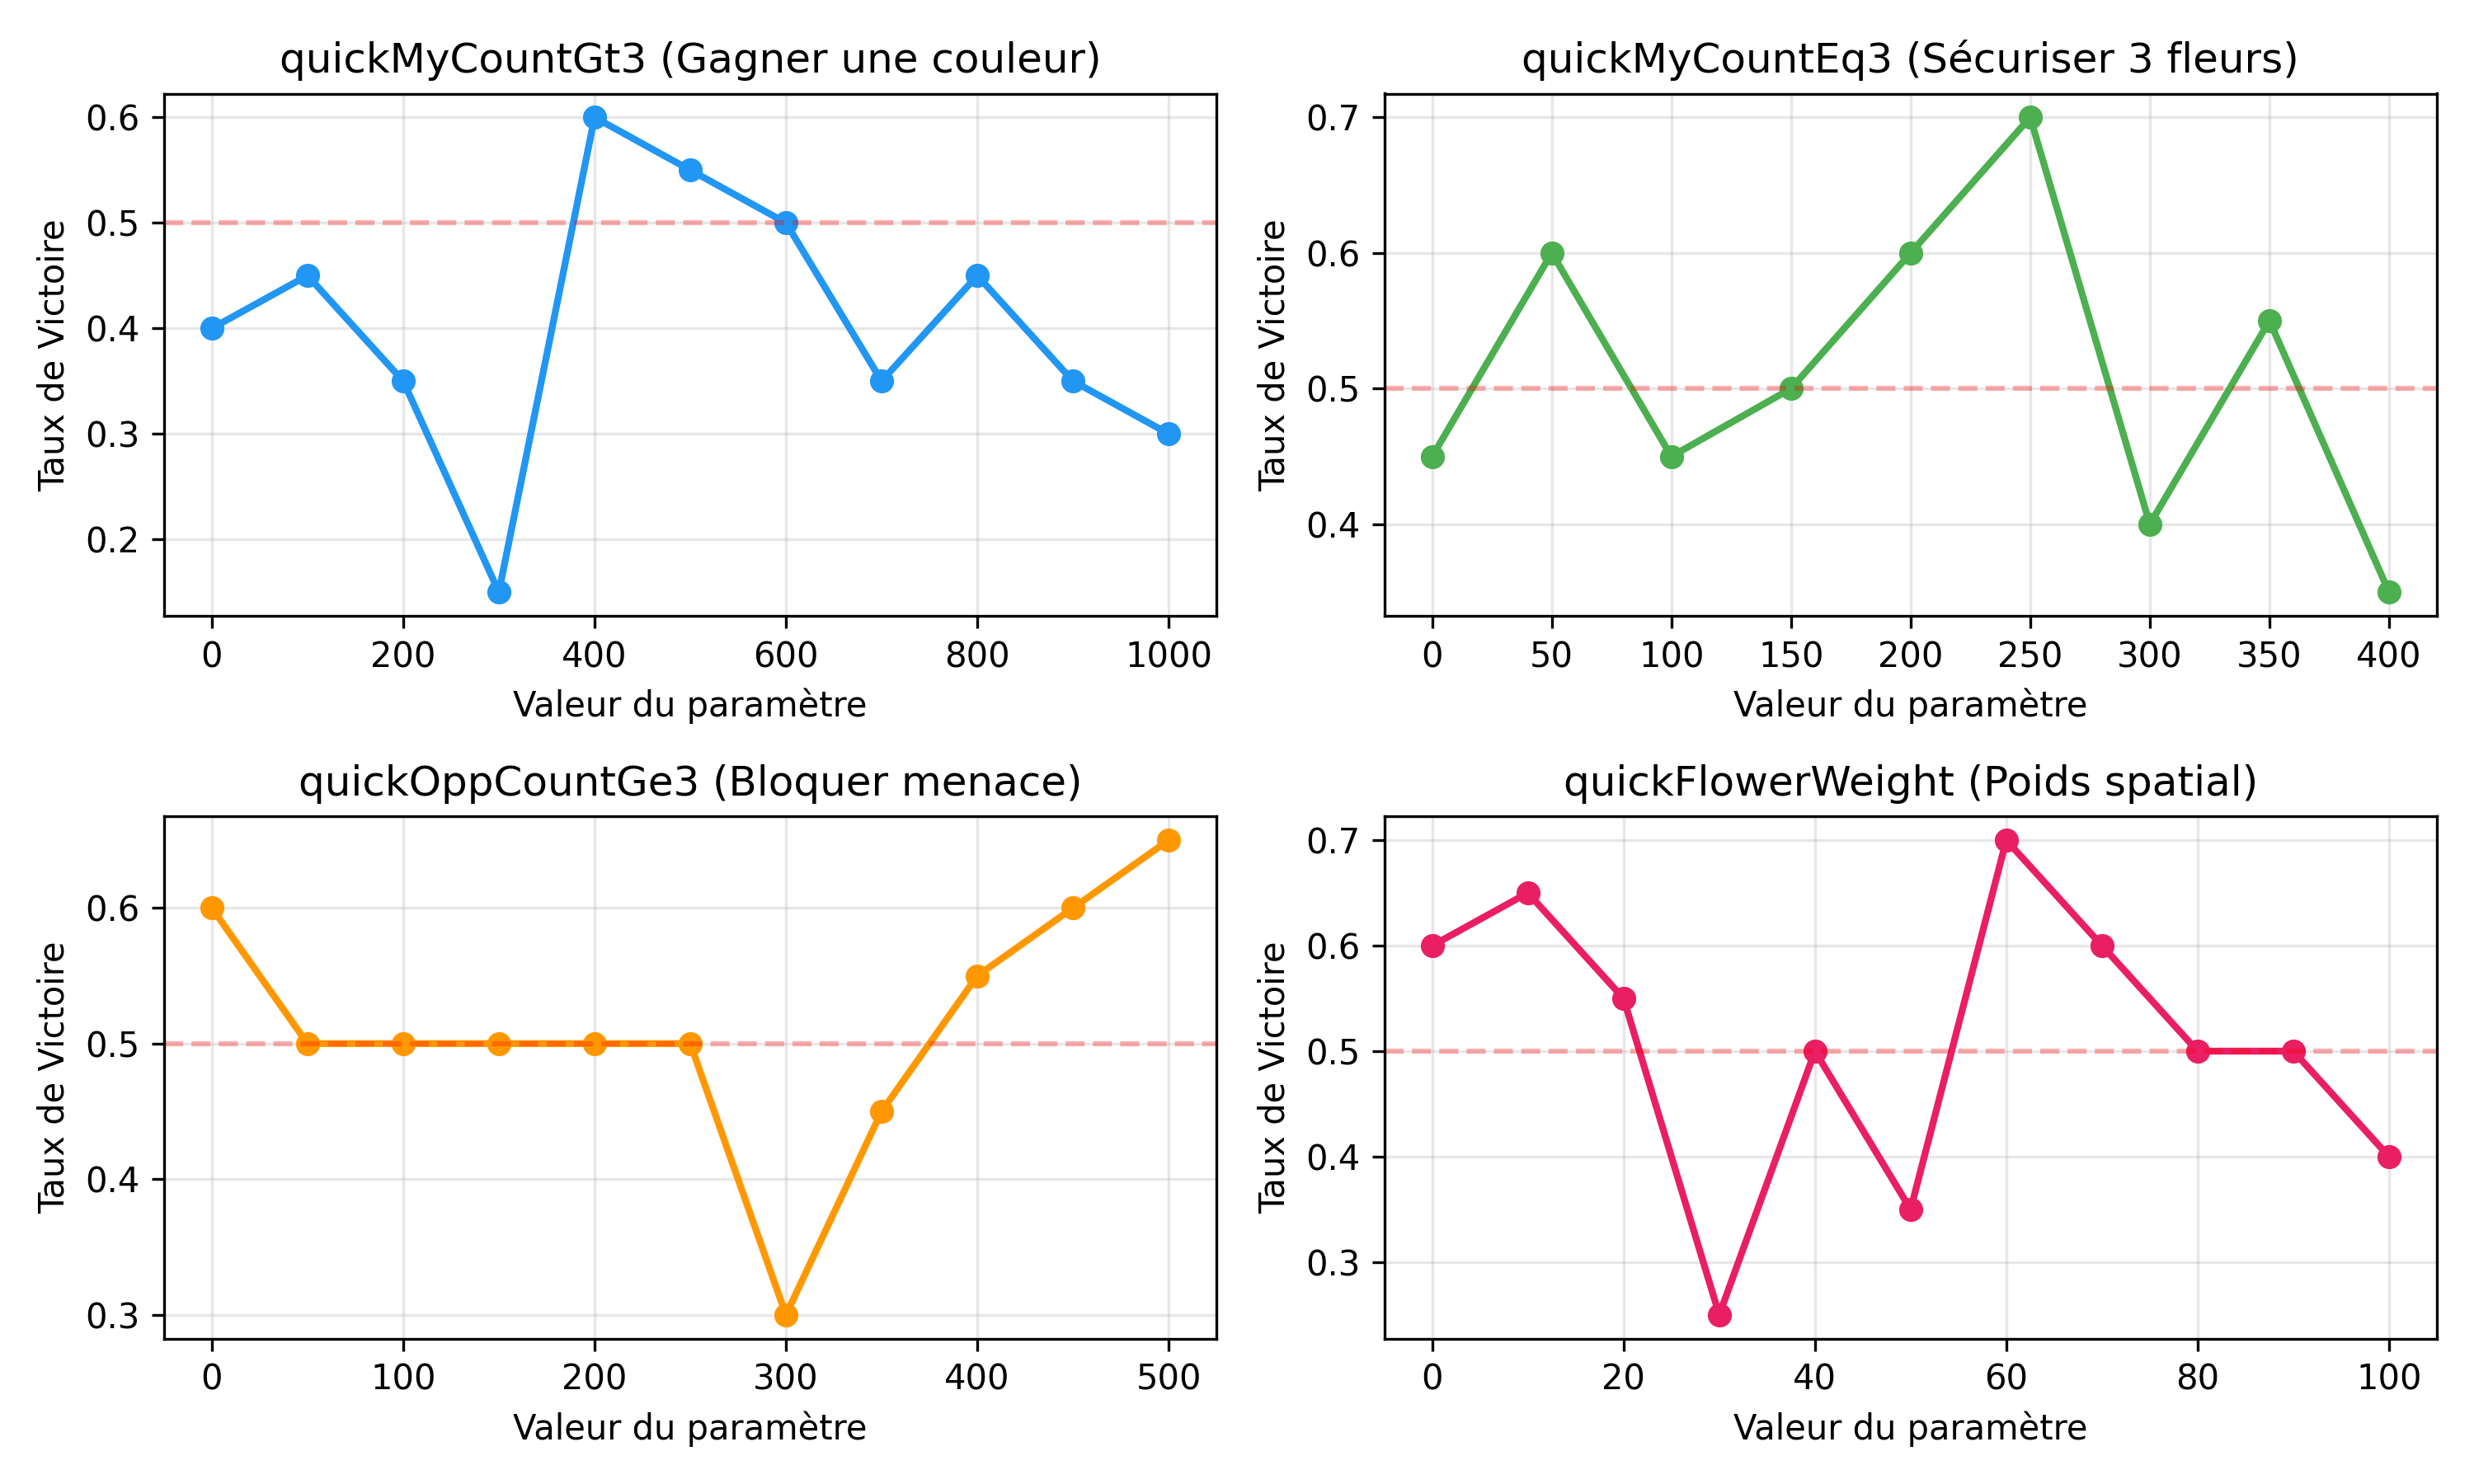
\includegraphics[width=0.75\textwidth]{tuning_quickeval.png}
    \caption{Impact du poids des param\`etres QuickEval sur le taux de victoire}
\end{figure}

Les graphiques empiriques confirment cette th\'eorie : des poids tr\`es faibles (0--500) pour le tri des menaces ne guident pas l'Alpha-Beta efficacement. En revanche, un poids de \textbf{10 000+} garantit l'analyse prioritaire des coups d\'efensifs critiques, rendant l'\'elagage maximal et s\'ecurisant la robustesse de l'IA.

% ======================================================================
\section{Validation : Les Niveaux de Difficulté}

\begin{figure}[H]
    \centering
    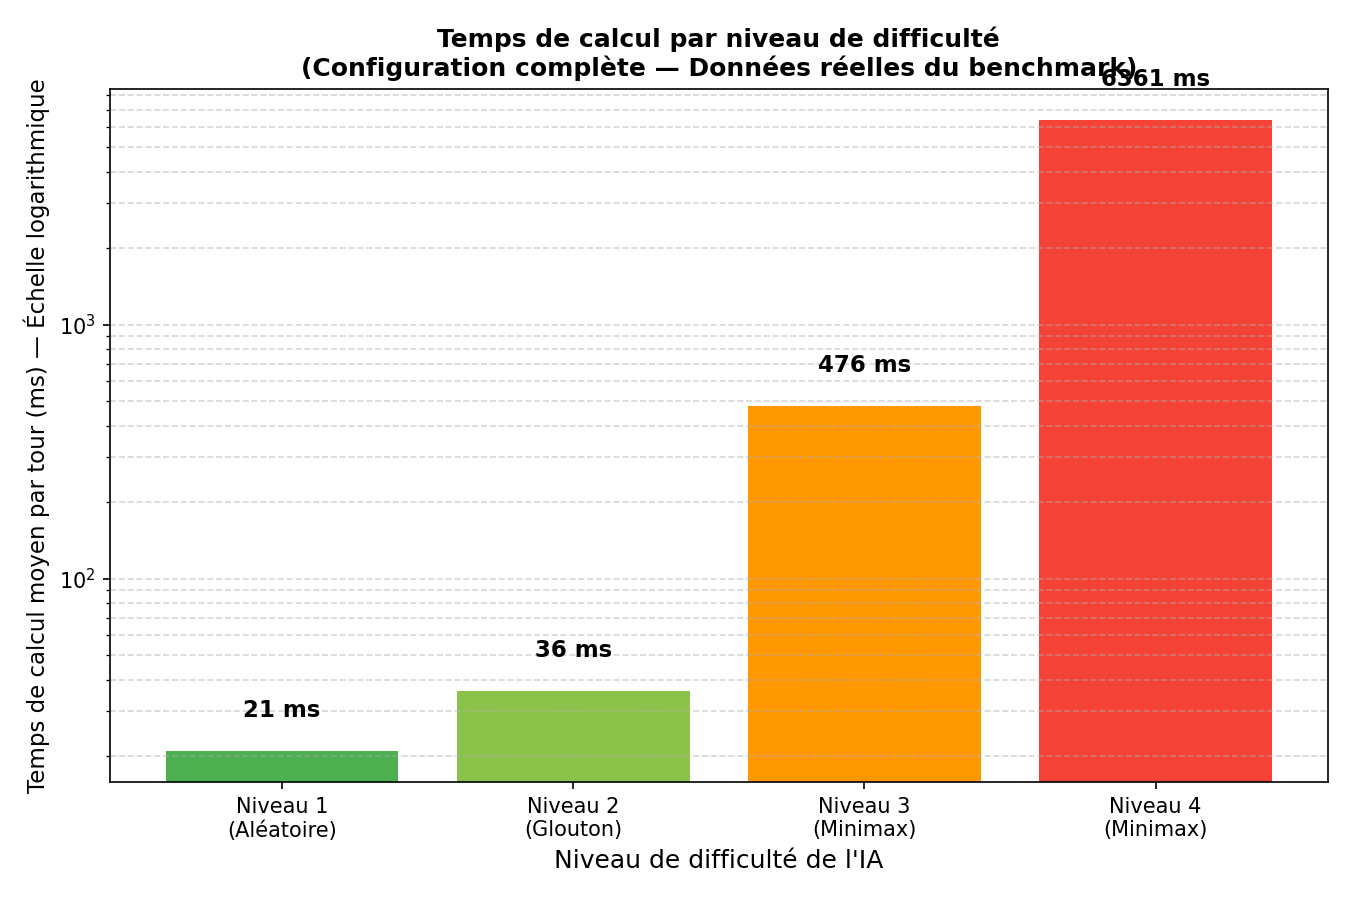
\includegraphics[width=0.8\textwidth]{difficulty_speed.png}
    \caption{Temps de calcul par niveau de difficulté (données réelles du benchmark)}
\end{figure}

\begin{itemize}
    \item \textbf{Niveau 1 (Aléatoire)} : $\sim 1$ ms. Taux de victoire de 0\% contre tous les autres niveaux. Sert à initier les débutants aux mécaniques du jeu.
    \item \textbf{Niveau 2 (Glouton)} : $\sim 20$ ms. Joue toujours le meilleur coup immédiat sans aucune anticipation. Facile à piéger sur 2 tours.
    \item \textbf{Niveau 3 (Minimax Prof. 3)} : $\sim 376$ ms. L'IA anticipe 3 demi-coups à l'avance et bat systématiquement le Niveau 2.
    \item \textbf{Niveau 4 (Minimax Prof. 4)} : $\sim 6343$ ms. La vraie IA. Anticipe 4 demi-coups. Lors de nos tests automatisés, le Niveau 4 bat le Niveau 3 dans environ \textbf{85\% des parties}.
\end{itemize}

% ======================================================================
\section{Conclusion}

L'IA de Lacuna a suivi une évolution architecturale rigoureuse. Le passage d'un simple échantillonnage de 5 points à une Descente de Gradient a amélioré la \textbf{précision} des coups, mais pas leur vitesse. La véritable explosion des performances est venue de l'introduction de la \textbf{Table de Transposition} (qui réduit le nombre de nœuds recalculés de plus de 55\%) et du \textbf{Tri Heuristique des Coups} (qui permet à l'élagage Alpha-Beta d'atteindre son efficacité maximale). L'ensemble de ces mécanismes a été affiné par un réglage empirique des paramètres heuristiques, aboutissant à un adversaire robuste, stratégique et imprévisible.

\end{document}
